\documentclass{article}

\usepackage{polski}
\usepackage[utf8]{inputenc}
\usepackage{indentfirst}
\usepackage{color}
\usepackage{graphicx}

\newcommand{\TODO}[1]{\textcolor{blue}{TODO: #1}}
\newcommand{\ang}[1]{ang.~{\itshape #1}}

\begin{document}

\title{Metody odkrywania wiedzy \\%
{\large Klasyfikacja -- założenia wstępne} }

\author{Jakub Cichanowicz \and Artur Sawicki}

\maketitle

\section{Interpretacja tematu projektu}
Nasz temat związany jest z tragedią Titanica z 1912 roku. Statek podczas swojego pierwszego rejsu zderzył się z górą lodową, co spowodowało jego zatonięcie oraz śmierć większości osób znajdujących się na nim.

Prawda jest taka, że o przeżyciu nie zdecydowało tylko szczęście, ale także inne parametry, takie jak: wiek, płeć czy przynależność do grupy społecznej.

Do dyspozycji mamy dane zawierające 891 obserwacji i na ich podstawie spróbujemy stwierdzić od jakich atrybutów i ich wartości zależało przeżycie w tej katastrofie.

\section{Opis algorytmów}
Do badań wykorzystane zostaną algorytmy zaimplementowane w różnych pakietach R. Planujemy wykonać następujące modele, należące do metod uczenia pod nadzorem.

\subsection{LDA}
LDA (\ang{Linear Discriminant Analysis}) -- celem tej metody jest określenie liniowej kombinacji cech, która pozwoli na najlepsze przyporządkowanie obserwacji do klas, w naszym przypadku dwóch. Przypuśćmy, że mamy macierz $p$ cech dla $N$ obserwacji $\mathbf{x}=(x_{1},...,x_{p})^{T}$. P-wymiarowe wektory rzutujemy na prostą określoną przez kierunek $w$. Cel analizy można osiągnąć poprzez wybór takiego kierunku $w$, który maksymalizuje odległości pomiędzy zrzutowanymi na $w$ średnimi dla klas jednocześnie minimalizując wariancję wewnątrz każdej z klas.

\subsection{Drzewo decyzyjne}
Metoda ta polega na utworzeniu modelu w postaci acyklicznego grafu skierowanego o strukturze drzewiastej na podstawie danych treningowych. Każdy wierzchołek reprezentuje test na atrybucie (bądź atrybutach), każda krawędź wynik testu, a każdy pojedynczy liść reprezentuje pojedynczą klasę lub rozkład wartości klas. Zbiór treningowy dzielony jest, w sposób rekurencyjny, na partycje, aż do momentu, w którym każda partycja zawiera dane należące do jednej klasy lub rozmiar partycji jest ograniczony. Każdy wierzchołek wewnętrzny drzewa jest tzw. punktem podziału, który dzieli zbiór danych na partycje. Oprócz fazy tworzenia drzewa wyróżnia się także fazę obcinania drzewa w celu poprawy dokładności modelu (identyfikowane są i usuwane gałęzie reprezentujące punkty osobliwe i szum). Zastosowanych zostanie kilka różnych algorytmów tworzenia drzewa, tj. CART, C5.0, CHAID, korzystających z różnych kryteriów podziału na partycje.

\subsection{Lasy losowe}
Jest to metoda wykorzystująca wiele mniejszych drzew decyzyjnych. Najpierw z danych treningowych losujemy $K$ zbiorów na podstawie których, konstruowane są drzewa decyzyjne w taki sposób, że w każdym węźle losujemy $m$ cech, które będą uczestniczyły w wyborze najlepszego podziału. Parametr $m$ powinien być znacznie mniejszy od liczby cech wystęujących w pojedynczym rekordzie danych trenujących. Drzewa budowane są bez przycinania. Ostatecznie
obserwacja klasyfikowana jest poprzez metodę głosowania.

\subsection{Naiwny klasyfikator Bayesa}

Zadaniem klasyfikatora Bayes’a, który jest statystycznym klasyfikatorem opartym na twierdzeniu Bayesa, jest przyporządkowanie nowego przypadku do jednej z klas decyzyjnych, przy czym zbiór klas decyzyjnych musi być skończony i zdefiniowany apriori. W celu zmniejszenia ilości obliczeń klasyfikator ten zakłada, że wartości atrybutów w klasach są niezależne. Założenie to jest zwane założeniem o niezależności warunkowej klasy (\ang{class conditional independence}). Naiwny klasyfikator Bayes’a opiera się na regule Bayes’a, zgodnie z którą przykład $X$ klasyfikujemy jako pochodzący z tej klasy $C_{i}$, dla której wartość $P(C_{i}|X)$, $i = 1, 2, ..., m$, jest największa.

\subsection{KNN}
Metoda $K$-najbliższych sąsiadów (\ang{K-nearest neighbors}) polega na klasyfikacji danej obserwacji na podstawie przynależności do klas jej $K$ najbliższych sąsiadów (według wybranej miary spełniającej konkretne założenia). Przykłady najczęściej wykorzystywanych miar: zwykła odległość euklidesowa, odległość miejska (taksówkowa) lub odległość Minkowskiego. Przebieg algorymu: iteracyjnie, dla każdej obserwacji zbioru testowego liczymy odległości od elementów zbioru treningowego, wybieramy $K$ najbliższych obserwacji i przypisujemy tę klasę, która wśród tych $K$ sąsiadów wystąpiła najczęściej. Liczba $K$ wybierana jest arbitrarnie przed wykonaniem modelu.

\section{Plan badań}

\subsection{Cel poszczególnych eksperymentów}

\TODO{Trochę nie wiem co tu wpisać:P}

\subsection{Charakterystyka zbioru danych}

W zbiorze danych mamy 12 zmiennych:
\begin{itemize}
\item Identyfikator pasażera ({\itshape PassengerId}) -- nie bierzemy jej pod uwagę, zmienna porządkowa;
\item Przeżycie ({\itshape Survived}) -- oznacza przeżycie danego pasażera, 0 - nie, 1 - tak, zmienna objaśniana;
\item Klasa pasażerska ({\itshape Pclass}) -- 1, 2 lub 3, nie ma braków danych, zmienna objaśniająca;
\item Imię i nazwisko z tytułem ({\itshape Name}) -- wstępnie wydaje nam się, że nie będziemy jej używać, jednak być może dałoby się jakoś z tego wyłączyć grupy ludzi po tytułach;
\item Płeć ({\itshape Sex}) -- nie ma braków danych, zmienna objaśniająca;
\item Wiek ({\itshape Age}) -- 177 braków, niektóre algorytmy sobie poradzą, inny sposób to dolosować, zastosujemy najprawdopodobniej oba podejścia, zmienna objaśniająca;
\item Liczba rodzeństwa/małżonków na pokładzie ({\itshape SibSp}) -- nie ma braków danych, zmienna objaśniająca;
\item Liczba dzieci/rodziców na pokładzie ({\itshape Parch}) -- nie ma braków danych, zmienna objaśniająca;
\item Numer biletu ({\itshape Ticket}) -- wstępnie wydaje się nieistotne, jednak być może będzie się dało jakoś pogrupować, być może przedrostki w biletach oznaczają jakieś częsci statku i będzie się dało to wykorzystać;
\item Opłata ({\itshape Fare}) -- nie ma braków danych, zmienna objaśniająca;
\item Kajuta ({\itshape Cabin}) -- 687 braków, spróbujemy wykorzystać obecność danych, aby lepiej klasyfikować osoby posiadające tę daną;
\item Miejsce wejścia na pokład ({\itshape Embarked}) -- nie wydaje się, żeby miało to znaczenie, ale może okazać się inaczej, zwłaszcza, że mamy bardzo mało braków, więc spróbujemy wykorzystać.
\end{itemize}

\subsection{Parametry algorytmów}

\TODO{Co tu wpsać - warunki stopu w tworzeniu drzew itp.?}

\subsection{Miary jakości i procedury oceny modeli}
Aby ocenić działanie poszczególnych modeli planujemy zestwić ze sobą klasy rzeczyiwiste dla części testowej naszych danych oraz klasy przewidziane przez modele.

\subsubsection{Macierz kontyngencji (macierz pomyłek)}
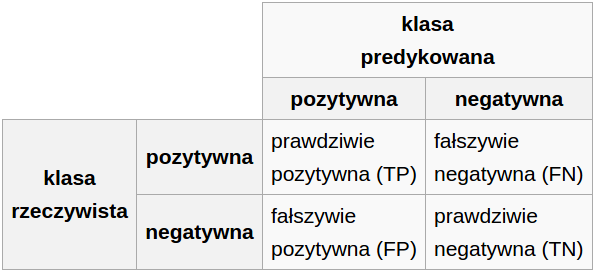
\includegraphics[scale=0.5]{../pictures/tablicaPomylek}\\

Na podstawie macierzy 2x2 możemy wyliczyć następujące wskaźniki:
\begin{itemize}
\item czułość (\ang{sensivity}): TPR=TP/(TP+FN)
\item specyficzność (\ang{specificity}): TNR=TN/(FP+TN)
\item precyzja (\ang{precision}): PR=TP/(TP+FP)
\item dokładność (\ang{accuracy}): ACC=(TP+TN)/(TP+TN+FP+FN)
\end{itemize}

W zależności od aspektu klasyfikacji, na którym nam najbardziej zależy (np. chcemy trafniej przewidywać ludzi którzy na pewno nie przeżyją) możemy porównywać ze sobą odpowiednie wartości.

\subsubsection{Krzywa ROC i miara AUC}
Krzywa ROC (\ang{Receiver Operating Characteristic}) jest dobrym graficznym sposobem na ocenę jakości modelu. Na wykresie przedstawiamy {\itshape czułość} -- oś Y -- w zależności od wartości {\itshape (1 -  specyficzność)} -- oś X. Im model lepiej przewiduje pożądaną klasę, tym szybciej powinna rosnąć funkcja ROC dla początkowych wartości na osi X. Dla modelu losowego krzywa ROC przyjmuje postać prostej.

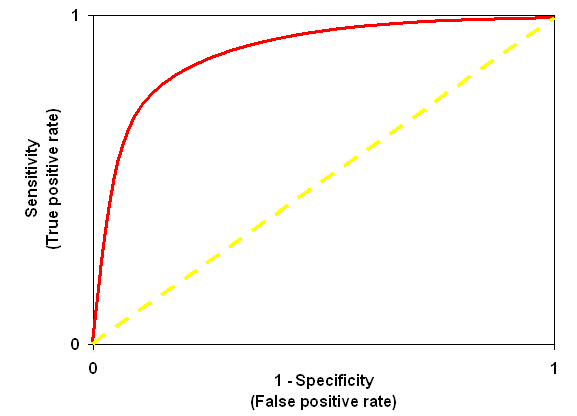
\includegraphics[scale=0.55]{../pictures/decoy4}\\

Miarą przydatną do porównywania modeli między sobą jest wskaźnik AUC (\ang{Area Under Curve}), który odpowiada wielkości pola pod krzywą ROC. Wskaźnik przybiera wartości od 0 do 1, gdzie 1 odpowiada modelowi idealnie przewidującemu klasy. Dla modelu losowego otrzymujemy wartość AUC=0.5.

\subsubsection{Walidacja krzyżowa}
Jako, że zbiór danych, na którym będziemy operować nie jest zbyt duży, wykorzystamy walidację krzyżową do oceny tworzonych modeli. Początkowy zbiór przykładów zostanie podzielony na $k$ możliwie równych, wzajemnie niezależnych części. Zbiór treningowy staniwić będą $k-1$ części, a $k$-ta część zbiór testowy. Każda z $k$ części będzie użyta $k-1$ razy do konstrukcji modelu i raz do testowania dokładności klasyfikacji. Sumaryczna liczba błędów klasyfikacji dla wszystkich $k$ klasyfikatorów, podzielona przez liczność $n$ oryginalnego zbioru przykładów daje kroswalidacyjne oszacowanie dokonania błędnej klasyfikacji przez dany klasyfikator.

\section{Otwarte kwestie}
\TODO{Pewnie ostatecznie to wywalimy - no chyba, że wymyśłimy co tu wpisać:P}

\end{document}
